\section{Cloud Grading Architecture With OpenEdX}
\label{sec:arch}

We adopt a narrow Unix-like view of an autograder: it is a
stateless command-line program that, given a student work submission and
a rubric, computes a score and some textual feedback.  We treat
separately the question of how to connect this program to a Learning
Management System (LMS).
All other policy issues---whether students can resubmit homeworks, how
late penalties are computed, where the gradebook is stored, and so 
on---are independent of the autograder\footnote{Due to an implementation
  artifact of OpenEdX, the autograders currently do adjust their scores
  to reflect late penalties, based on metadata about due dates provided
  with each assignment submission.}, as is the question of whether these
autograders should replace or supplement manual grading by instructors.
While these issues are pedagogically important, for engineering purposes
we declare them strictly outside the scope of the autograder code itself.

\subsection{Why Another Autograder?}

Given that 17 autograding systems and over 60 papers about them were
produced from 2006--2010 alone~\cite{ihantola-2010-autograding-survey},
why did we choose to build our own?
First, as the survey authors point
out, many existing systems' code
is not readily available or is tightly integrated to a particular Learning
Management System (LMS).  We needed to integrate with Coursera and
later OpenEdX, both of which were new and had not yet embraced
standards such as Learning Tools Interoperability\uf{imsglobal.org/lti}.
Unlike most previous 
systems, ours would need to work at ``cloud scale'' and respond to
workload spikes: the initial
offering of our MOOC in February 2012  
attracted over 50,000 learners, and we expected
that thousands of submissions would arrive bunched together close to the
submission deadline.  For the same reason, our graders needed to be
highly insulated from the LMS, so that students whose code accidentally
or deliberately damaged the autograder could not compromise other
information in the LMS.
Similarly, 
%% with a diverse and international group (less than
%% 25\% of our MOOC learners were from the USA) with varied hardware,
%% software, and operating systems, autograding had to be ``zero
%% configuration,'' requiring no installation of software on learners' own
%% computers, and 
the autograders had to be trustworthy, in that the student
assignments were authoritatively graded on trusted servers rather than
having students self-report grades computed by their own computers
(although of course we still have no guarantee that students are doing
their own work).


\subsection{Student Experience and Cloud Grading Architecture}

\begin{figure}
  \centering
  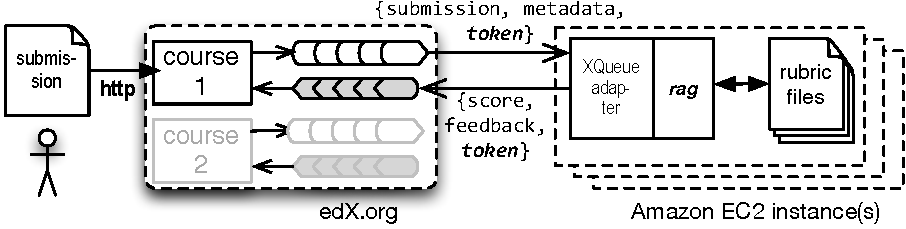
\includegraphics[width=\textwidth]{figs/autograder_arch.pdf}
  \caption{\label{fig:autograder_arch}
  Since MAGIC relies on many libraries,
  tools, support files, and so on, we encapsulate it in a
  virtual machine image that is deployed on Amazon Elastic Compute Cloud.
  When a new instance is started, the autograder script automatically runs from
  \texttt{/etc/init.d} and examines a deploy-time environment variable
  to obtain the credentials needed to make calls to the XQueues.}
\end{figure}


Our initial implementation of autograding was designed to work with
Coursera and later adapted to OpenEdX.  Both the API and the student
experience are similar 
between the two.  A logged-in student navigates to a page
containing instructions and handouts for a homework assignment;
when ready, the learner submits a single file or a
\texttt{tar} or \texttt{zip} archive through a standard HTTP
file-upload form.  A short time later, typically less than a minute, the
student can refresh the page to see feedback on her work from the
autograder.  

As Figure~\ref{fig:autograder_arch} shows, 
the student's submitted file, plus
submission metadata specified at course authoring time, go into a
persistent queue in the OpenEdX server; each course has its own queue.
We use the metadata field to distinguish different
assignments so that the autograder knows which engine and rubric files
must be used to grade that assignment.
The OpenEdX LMS defines an authenticated RESTful
API\uf{edx-partner-course-staff.readthedocs.org/en/latest/exercises\_tools/external\_graders.html}
by which external standalone autograders can retrieve student
submissions from these queues and later post back a numerical grade and
textual feedback.
The external grader does not have access to the identity of the learner;
instead, an obfuscated token identifies the learner, with the mappings
to the learners' true identities maintained only on OpenEdX.
Hence no sensitive information connecting a work product to a specific
student is leaked if the autograder is compromised.
%% Retrieving an
%% assignment and posting back a 
%% grade are separate queue operations, to allow for autograders that may
%% take a long time to run.  
%% If the autograder polls the XQueue and finds it empty, the grader
%% process sleeps for awhile and tries again.  (In the future we will allow
%% idle autograders to kill themselves.)
Once a submission is retrieved from the queue, the metadata identifies
which grader engine and instructor-supplied rubric files (described
subsequently) should be 
used to grade the assignment.  
The engine itself, \emph{rag}\/ (Ruby AutoGrader), is essentially a Unix
command-line program that consumes the submission filename and rubric
filename(s) as command-line arguments and produces a numerical score
(normalized to 100 points) and freeform text feedback.  The XQueueAdapter
in the figure is a wrapper around this program that retrieves the
submission from OpenEdX and posts the numerical score and feedback
(formatted as a JSON object) back to OpenEdX.

This simple architecture keeps the grader process stateless, thereby 
simplifying the implementation of cloud-based graders in three ways:

\noindent\textbf{1. No data loss.}
If an assignment is retrieved but no grade is posted back before
a pre-set timeout, OpenEdX eventually returns the ungraded assignment to
the queue, where it will presumably be picked up again by another
autograder instance.
Therefore, if an autograder crashes while grading an assignment, no
student work is lost.

\noindent\textbf{2. Scale-out.} 
Since the autograders are stateless consumers
contacting a single producer (the queue), and grading is
embarrassingly task-parallel, we can drain the queues faster by simply
deploying additional autograder instances.
Since we package the entire autograder and supporting libraries as a
virtual machine image deployed on Amazon's cloud, deploying an
additional grader is essentially a one-click operation. (We have not
yet had the time to automate scaling and provisioning.)
\footnote{OpenEdX also supports an alternative ``push'' protocol in which each student
submission event triggers a call to a RESTful autograder endpoint.
We do not use this
alternative protocol because it thwarts this simple scaling technique
and because we would be  unable to limit the rate at which
submissions were pushed to our autograders during peak times.}
Even our most sophisticated autograders take less than one
machine-minute per assignment, so at less than 10 cents per machine-hour,
MOOC-scale 
autograding is cost-effective and fast: even with
thousands of assignments being submitted in a 50,000-learner course,
students rarely waited more than a few minutes to get feedback, and we
can grade over 1,000 assignments for US~\$1.

\noindent\textbf{3. Crash-only design~\cite{candea:crash-only}.}
If the external grader crashes (which it does periodically), it can
simply be restarted, which we in fact do in the
body of a \texttt{while(true)} shell script.
If the entire VM becomes unresponsive, for example if it becomes
corrupted by misbehaving student code, it can be rebooted or
undeployed as needed, with no data loss.

In short, the simple external grader architecture of OpenEdX provides a
good separation 
of concerns between the LMS and autograder authors.

\subsection{CI Workflow for Autograders}

Since at any given time the autograders
may be in use by the MOOC and several campus SPOCs (Small Private Online
Courses~\cite{spoc}), it is important to 
avoid introducing breaking changes to rubric files, homework
assignments, or the autograders themselves.
We set up continuous
integration tasks using Travis-CI, which is integrated with GitHub.
When a pull request is made\footnote{A pull request is
  GitHub's term for the mechanism by which a developer requests that a
  set of changes 
  be merged into the production branch of a codebase.},  
the CI task instantiates  a
new virtual 
machine, installs all the needed software to build an autograder image
based on the codebase as it would appear after the pull request,
and tests the autograder with known solutions versioned with each homework, as
Figure~\ref{fig:rag-ci} shows.
%% These CI features run the autograders locally against
%% inputs via the Open3 library in order to control output streams and
%% return codes. 
Each homework assignment repository also has a CI task that
automates the installation of the autograders and verifies their
configuration. 

%% \begin{figure}[!htbp]
%%   \centering
%%   \begin{minipage}{0.70\textwidth}%
%%   \lstset{tabsize=1,basicstyle=\scriptsize\ttfamily}%
%%   \lstinputlisting{figs/travis.yml}%
%%   \end{minipage}
%%   \caption{\label{fig:rag-ci}%
%%   Typical .travis.yml file.
%% }
%% \end{figure}

\begin{figure}
  \centering
  \lstinputlisting[tabsize=1,basicstyle=\scriptsize\ttfamily]{figs/ci_feature.txt}%
  \lstinputlisting[tabsize=1,language=Ruby,basicstyle=\scriptsize\ttfamily]{figs/ci_stepdefs.rb}%
  \caption{\label{fig:rag-ci}%
  Top: Cucumber integration test that is run whenever the autograder or
  homework code is updated.  (Cucumber is described in the next
  section.)
  The scenarios verify that, at a minimum,
  the autograder reports a score of 100\% when run against the
  instructor's reference solution and a score of 0\% when run against
  the empty ``code skeleton'' provided to students.  
  Bottom: examples of the Cucumber step definitions invoked when these
  steps are run.
}
\end{figure}

